\documentclass[1p]{elsarticle_modified}
%\bibliographystyle{elsarticle-num}

%\usepackage[colorlinks]{hyperref}
%\usepackage{abbrmath_seonhwa} %\Abb, \Ascr, \Acal ,\Abf, \Afrak
\usepackage{amsfonts}
\usepackage{amssymb}
\usepackage{amsmath}
\usepackage{amsthm}
\usepackage{scalefnt}
\usepackage{amsbsy}
\usepackage{kotex}
\usepackage{caption}
\usepackage{subfig}
\usepackage{color}
\usepackage{graphicx}
\usepackage{xcolor} %% white, black, red, green, blue, cyan, magenta, yellow
\usepackage{float}
\usepackage{setspace}
\usepackage{hyperref}

\usepackage{tikz}
\usetikzlibrary{arrows}

\usepackage{multirow}
\usepackage{array} % fixed length table
\usepackage{hhline}

%%%%%%%%%%%%%%%%%%%%%
\makeatletter
\renewcommand*\env@matrix[1][\arraystretch]{%
	\edef\arraystretch{#1}%
	\hskip -\arraycolsep
	\let\@ifnextchar\new@ifnextchar
	\array{*\c@MaxMatrixCols c}}
\makeatother %https://tex.stackexchange.com/questions/14071/how-can-i-increase-the-line-spacing-in-a-matrix
%%%%%%%%%%%%%%%

\usepackage[normalem]{ulem}

\newcommand{\msout}[1]{\ifmmode\text{\sout{\ensuremath{#1}}}\else\sout{#1}\fi}
%SOURCE: \msout is \stkout macro in https://tex.stackexchange.com/questions/20609/strikeout-in-math-mode

\newcommand{\cancel}[1]{
	\ifmmode
	{\color{red}\msout{#1}}
	\else
	{\color{red}\sout{#1}}
	\fi
}

\newcommand{\add}[1]{
	{\color{blue}\uwave{#1}}
}

\newcommand{\replace}[2]{
	\ifmmode
	{\color{red}\msout{#1}}{\color{blue}\uwave{#2}}
	\else
	{\color{red}\sout{#1}}{\color{blue}\uwave{#2}}
	\fi
}

\newcommand{\Sol}{\mathcal{S}} %segment
\newcommand{\D}{D} %diagram
\newcommand{\A}{\mathcal{A}} %arc


%%%%%%%%%%%%%%%%%%%%%%%%%%%%%5 test

\def\sl{\operatorname{\textup{SL}}(2,\Cbb)}
\def\psl{\operatorname{\textup{PSL}}(2,\Cbb)}
\def\quan{\mkern 1mu \triangleright \mkern 1mu}

\theoremstyle{definition}
\newtheorem{thm}{Theorem}[section]
\newtheorem{prop}[thm]{Proposition}
\newtheorem{lem}[thm]{Lemma}
\newtheorem{ques}[thm]{Question}
\newtheorem{cor}[thm]{Corollary}
\newtheorem{defn}[thm]{Definition}
\newtheorem{exam}[thm]{Example}
\newtheorem{rmk}[thm]{Remark}
\newtheorem{alg}[thm]{Algorithm}

\newcommand{\I}{\sqrt{-1}}
\begin{document}

%\begin{frontmatter}
%
%\title{Boundary parabolic representations of knots up to 8 crossings}
%
%%% Group authors per affiliation:
%\author{Yunhi Cho} 
%\address{Department of Mathematics, University of Seoul, Seoul, Korea}
%\ead{yhcho@uos.ac.kr}
%
%
%\author{Seonhwa Kim} %\fnref{s_kim}}
%\address{Center for Geometry and Physics, Institute for Basic Science, Pohang, 37673, Korea}
%\ead{ryeona17@ibs.re.kr}
%
%\author{Hyuk Kim}
%\address{Department of Mathematical Sciences, Seoul National University, Seoul 08826, Korea}
%\ead{hyukkim@snu.ac.kr}
%
%\author{Seokbeom Yoon}
%\address{Department of Mathematical Sciences, Seoul National University, Seoul, 08826,  Korea}
%\ead{sbyoon15@snu.ac.kr}
%
%\begin{abstract}
%We find all boundary parabolic representation of knots up to 8 crossings.
%
%\end{abstract}
%\begin{keyword}
%    \MSC[2010] 57M25 
%\end{keyword}
%
%\end{frontmatter}

%\linenumbers
%\tableofcontents
%
\newcommand\colored[1]{\textcolor{white}{\rule[-0.35ex]{0.8em}{1.4ex}}\kern-0.8em\color{red} #1}%
%\newcommand\colored[1]{\textcolor{white}{ #1}\kern-2.17ex	\textcolor{white}{ #1}\kern-1.81ex	\textcolor{white}{ #1}\kern-2.15ex\color{red}#1	}

{\Large $\underline{12a_{1245}~(K12a_{1245})}$}

\setlength{\tabcolsep}{10pt}
\renewcommand{\arraystretch}{1.6}
\vspace{1cm}\begin{tabular}{m{100pt}>{\centering\arraybackslash}m{274pt}}
\multirow{5}{120pt}{
	\centering
	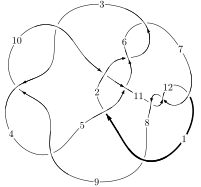
\includegraphics[width=112pt]{../../../GIT/diagram.site/Diagrams/png/2046_12a_1245.png}\\
\ \ \ A knot diagram\footnotemark}&
\allowdisplaybreaks
\textbf{Linearized knot diagam} \\
\cline{2-2}
 &
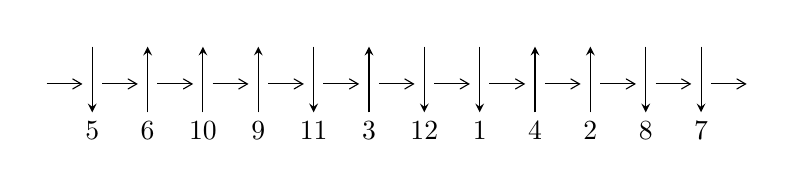
\begin{tikzpicture}[x=20pt, y=17pt]
	% nodes
	\node (C0) at (0, 0) {};
	\node (C1) at (1, 0) {};
	\node (C1U) at (1, +1) {};
	\node (C1D) at (1, -1) {5};

	\node (C2) at (2, 0) {};
	\node (C2U) at (2, +1) {};
	\node (C2D) at (2, -1) {6};

	\node (C3) at (3, 0) {};
	\node (C3U) at (3, +1) {};
	\node (C3D) at (3, -1) {10};

	\node (C4) at (4, 0) {};
	\node (C4U) at (4, +1) {};
	\node (C4D) at (4, -1) {9};

	\node (C5) at (5, 0) {};
	\node (C5U) at (5, +1) {};
	\node (C5D) at (5, -1) {11};

	\node (C6) at (6, 0) {};
	\node (C6U) at (6, +1) {};
	\node (C6D) at (6, -1) {3};

	\node (C7) at (7, 0) {};
	\node (C7U) at (7, +1) {};
	\node (C7D) at (7, -1) {12};

	\node (C8) at (8, 0) {};
	\node (C8U) at (8, +1) {};
	\node (C8D) at (8, -1) {1};

	\node (C9) at (9, 0) {};
	\node (C9U) at (9, +1) {};
	\node (C9D) at (9, -1) {4};

	\node (C10) at (10, 0) {};
	\node (C10U) at (10, +1) {};
	\node (C10D) at (10, -1) {2};

	\node (C11) at (11, 0) {};
	\node (C11U) at (11, +1) {};
	\node (C11D) at (11, -1) {8};

	\node (C12) at (12, 0) {};
	\node (C12U) at (12, +1) {};
	\node (C12D) at (12, -1) {7};
	\node (C13) at (13, 0) {};

	% arrows
	\draw[->,>={angle 60}]
	(C0) edge (C1) (C1) edge (C2) (C2) edge (C3) (C3) edge (C4) (C4) edge (C5) (C5) edge (C6) (C6) edge (C7) (C7) edge (C8) (C8) edge (C9) (C9) edge (C10) (C10) edge (C11) (C11) edge (C12) (C12) edge (C13) ;	\draw[->,>=stealth]
	(C1U) edge (C1D) (C2D) edge (C2U) (C3D) edge (C3U) (C4D) edge (C4U) (C5U) edge (C5D) (C6D) edge (C6U) (C7U) edge (C7D) (C8U) edge (C8D) (C9D) edge (C9U) (C10D) edge (C10U) (C11U) edge (C11D) (C12U) edge (C12D) ;
	\end{tikzpicture} \\
\hhline{~~} \\& 
\textbf{Solving Sequence} \\ \cline{2-2} 
 &
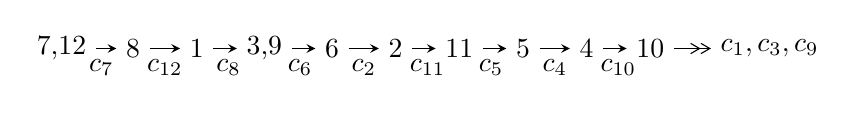
\begin{tikzpicture}[x=23pt, y=7pt]
	% node
	\node (A0) at (-1/8, 0) {7,12};
	\node (A1) at (1, 0) {8};
	\node (A2) at (2, 0) {1};
	\node (A3) at (49/16, 0) {3,9};
	\node (A4) at (33/8, 0) {6};
	\node (A5) at (41/8, 0) {2};
	\node (A6) at (49/8, 0) {11};
	\node (A7) at (57/8, 0) {5};
	\node (A8) at (65/8, 0) {4};
	\node (A9) at (73/8, 0) {10};
	\node (C1) at (1/2, -1) {$c_{7}$};
	\node (C2) at (3/2, -1) {$c_{12}$};
	\node (C3) at (5/2, -1) {$c_{8}$};
	\node (C4) at (29/8, -1) {$c_{6}$};
	\node (C5) at (37/8, -1) {$c_{2}$};
	\node (C6) at (45/8, -1) {$c_{11}$};
	\node (C7) at (53/8, -1) {$c_{5}$};
	\node (C8) at (61/8, -1) {$c_{4}$};
	\node (C9) at (69/8, -1) {$c_{10}$};
	\node (A10) at (11, 0) {$c_{1},c_{3},c_{9}$};

	% edge
	\draw[->,>=stealth]	
	(A0) edge (A1) (A1) edge (A2) (A2) edge (A3) (A3) edge (A4) (A4) edge (A5) (A5) edge (A6) (A6) edge (A7) (A7) edge (A8) (A8) edge (A9) ;
	\draw[->>,>={angle 60}]	
	(A9) edge (A10);
\end{tikzpicture} \\ 

\end{tabular} \\

\footnotetext{
The image of knot diagram is generated by the software ``\textbf{Draw programme}" developed by Andrew Bartholomew(\url{http://www.layer8.co.uk/maths/draw/index.htm\#Running-draw}), where we modified some parts for our purpose(\url{https://github.com/CATsTAILs/LinksPainter}).
}\phantom \\ \newline 
\centering \textbf{Ideals for irreducible components\footnotemark of $X_{\text{par}}$} 
 
\begin{align*}
I^u_{1}&=\langle 
-3.10423\times10^{148} u^{106}-7.11831\times10^{147} u^{105}+\cdots+4.99479\times10^{148} b-4.54934\times10^{149},\\
\phantom{I^u_{1}}&\phantom{= \langle  }1.94237\times10^{149} u^{106}+4.11737\times10^{149} u^{105}+\cdots+9.49010\times10^{149} a+6.20020\times10^{150},\\
\phantom{I^u_{1}}&\phantom{= \langle  }u^{107}+47 u^{105}+\cdots+141 u+19\rangle \\
I^u_{2}&=\langle 
- u^{18}- u^{17}+\cdots+b+1,\;- u^{20}-3 u^{19}+\cdots+a+2,\;u^{21}+u^{20}+\cdots-2 u-1\rangle \\
\\
\end{align*}
\raggedright * 2 irreducible components of $\dim_{\mathbb{C}}=0$, with total 128 representations.\\
\footnotetext{All coefficients of polynomials are rational numbers. But the coefficients are sometimes approximated in decimal forms when there is not enough margin.}
\newpage
\renewcommand{\arraystretch}{1}
\centering \section*{I. $I^u_{1}= \langle -3.10\times10^{148} u^{106}-7.12\times10^{147} u^{105}+\cdots+4.99\times10^{148} b-4.55\times10^{149},\;1.94\times10^{149} u^{106}+4.12\times10^{149} u^{105}+\cdots+9.49\times10^{149} a+6.20\times10^{150},\;u^{107}+47 u^{105}+\cdots+141 u+19 \rangle$}
\flushleft \textbf{(i) Arc colorings}\\
\begin{tabular}{m{7pt} m{180pt} m{7pt} m{180pt} }
\flushright $a_{7}=$&$\begin{pmatrix}1\\0\end{pmatrix}$ \\
\flushright $a_{12}=$&$\begin{pmatrix}0\\u\end{pmatrix}$ \\
\flushright $a_{8}=$&$\begin{pmatrix}1\\u^2\end{pmatrix}$ \\
\flushright $a_{1}=$&$\begin{pmatrix}- u\\u\end{pmatrix}$ \\
\flushright $a_{3}=$&$\begin{pmatrix}-0.204673 u^{106}-0.433859 u^{105}+\cdots-46.4584 u-6.53333\\0.621494 u^{106}+0.142515 u^{105}+\cdots+61.8909 u+9.10817\end{pmatrix}$ \\
\flushright $a_{9}=$&$\begin{pmatrix}- u^4- u^2+1\\u^4+2 u^2\end{pmatrix}$ \\
\flushright $a_{6}=$&$\begin{pmatrix}-0.106621 u^{106}+1.50979 u^{105}+\cdots+122.935 u+18.4439\\-1.10574 u^{106}-0.316137 u^{105}+\cdots-140.594 u-23.7789\end{pmatrix}$ \\
\flushright $a_{2}=$&$\begin{pmatrix}-0.700162 u^{106}+1.60344 u^{105}+\cdots+21.6036 u-3.11076\\-0.791948 u^{106}-1.19829 u^{105}+\cdots-211.859 u-36.8786\end{pmatrix}$ \\
\flushright $a_{11}=$&$\begin{pmatrix}u\\u^3+u\end{pmatrix}$ \\
\flushright $a_{5}=$&$\begin{pmatrix}0.0653729 u^{106}+0.714844 u^{105}+\cdots+58.6773 u+8.36870\\-0.839895 u^{106}+0.179953 u^{105}+\cdots-96.0311 u-18.7501\end{pmatrix}$ \\
\flushright $a_{4}=$&$\begin{pmatrix}0.508771 u^{106}+1.70694 u^{105}+\cdots+210.070 u+33.7699\\-1.31324 u^{106}-0.319179 u^{105}+\cdots-135.759 u-21.9463\end{pmatrix}$ \\
\flushright $a_{10}=$&$\begin{pmatrix}-0.451438 u^{106}+0.642648 u^{105}+\cdots-59.0515 u-15.1553\\-0.610494 u^{106}-0.619999 u^{105}+\cdots-144.993 u-26.1983\end{pmatrix}$\\&\end{tabular}
\flushleft \textbf{(ii) Obstruction class $= -1$}\\~\\
\flushleft \textbf{(iii) Cusp Shapes $= 0.227553 u^{106}-0.275413 u^{105}+\cdots-161.851 u-42.6015$}\\~\\
\newpage\renewcommand{\arraystretch}{1}
\flushleft \textbf{(iv) u-Polynomials at the component}\newline \\
\begin{tabular}{m{50pt}|m{274pt}}
Crossings & \hspace{64pt}u-Polynomials at each crossing \\
\hline $$\begin{aligned}c_{1}\end{aligned}$$&$\begin{aligned}
&u^{107}+7 u^{106}+\cdots-3628491 u-687859
\end{aligned}$\\
\hline $$\begin{aligned}c_{2},c_{6}\end{aligned}$$&$\begin{aligned}
&u^{107}+2 u^{106}+\cdots-142 u+7
\end{aligned}$\\
\hline $$\begin{aligned}c_{3},c_{4},c_{9}\end{aligned}$$&$\begin{aligned}
&u^{107}+u^{106}+\cdots+43 u+1
\end{aligned}$\\
\hline $$\begin{aligned}c_{5}\end{aligned}$$&$\begin{aligned}
&u^{107}+u^{106}+\cdots+229 u+31
\end{aligned}$\\
\hline $$\begin{aligned}c_{7},c_{11},c_{12}\end{aligned}$$&$\begin{aligned}
&u^{107}+47 u^{105}+\cdots+141 u+19
\end{aligned}$\\
\hline $$\begin{aligned}c_{8}\end{aligned}$$&$\begin{aligned}
&u^{107}-21 u^{105}+\cdots+516631 u+130055
\end{aligned}$\\
\hline $$\begin{aligned}c_{10}\end{aligned}$$&$\begin{aligned}
&u^{107}-7 u^{106}+\cdots+u+1
\end{aligned}$\\
\hline
\end{tabular}\\~\\
\newpage\renewcommand{\arraystretch}{1}
\flushleft \textbf{(v) Riley Polynomials at the component}\newline \\
\begin{tabular}{m{50pt}|m{274pt}}
Crossings & \hspace{64pt}Riley Polynomials at each crossing \\
\hline $$\begin{aligned}c_{1}\end{aligned}$$&$\begin{aligned}
&y^{107}-25 y^{106}+\cdots+17280320516861 y-473150003881
\end{aligned}$\\
\hline $$\begin{aligned}c_{2},c_{6}\end{aligned}$$&$\begin{aligned}
&y^{107}-62 y^{106}+\cdots+4890 y-49
\end{aligned}$\\
\hline $$\begin{aligned}c_{3},c_{4},c_{9}\end{aligned}$$&$\begin{aligned}
&y^{107}+109 y^{106}+\cdots+1159 y-1
\end{aligned}$\\
\hline $$\begin{aligned}c_{5}\end{aligned}$$&$\begin{aligned}
&y^{107}+15 y^{106}+\cdots-27601 y-961
\end{aligned}$\\
\hline $$\begin{aligned}c_{7},c_{11},c_{12}\end{aligned}$$&$\begin{aligned}
&y^{107}+94 y^{106}+\cdots+6619 y-361
\end{aligned}$\\
\hline $$\begin{aligned}c_{8}\end{aligned}$$&$\begin{aligned}
&y^{107}-42 y^{106}+\cdots+181397207991 y-16914303025
\end{aligned}$\\
\hline $$\begin{aligned}c_{10}\end{aligned}$$&$\begin{aligned}
&y^{107}+y^{106}+\cdots+111 y-1
\end{aligned}$\\
\hline
\end{tabular}\\~\\
\newpage\flushleft \textbf{(vi) Complex Volumes and Cusp Shapes}
$$\begin{array}{c|c|c}  
\text{Solutions to }I^u_{1}& \I (\text{vol} + \sqrt{-1}CS) & \text{Cusp shape}\\
 \hline 
\begin{aligned}
u &= \phantom{-}0.905238 + 0.411449 I \\
a &= -1.096800 - 0.625171 I \\
b &= \phantom{-}0.733290 - 0.222077 I\end{aligned}
 & -7.44404 - 2.71116 I & \phantom{-0.000000 } 0 \\ \hline\begin{aligned}
u &= \phantom{-}0.905238 - 0.411449 I \\
a &= -1.096800 + 0.625171 I \\
b &= \phantom{-}0.733290 + 0.222077 I\end{aligned}
 & -7.44404 + 2.71116 I & \phantom{-0.000000 } 0 \\ \hline\begin{aligned}
u &= \phantom{-}0.968712 + 0.181097 I \\
a &= -0.0104473 + 0.1331340 I \\
b &= \phantom{-}0.937029 + 0.334740 I\end{aligned}
 & -6.63928 - 0.01925 I & \phantom{-0.000000 } 0 \\ \hline\begin{aligned}
u &= \phantom{-}0.968712 - 0.181097 I \\
a &= -0.0104473 - 0.1331340 I \\
b &= \phantom{-}0.937029 - 0.334740 I\end{aligned}
 & -6.63928 + 0.01925 I & \phantom{-0.000000 } 0 \\ \hline\begin{aligned}
u &= -0.364131 + 0.957400 I \\
a &= -1.067810 + 0.496371 I \\
b &= \phantom{-}0.302228 + 1.008320 I\end{aligned}
 & -7.21376 - 2.28542 I & \phantom{-0.000000 } 0 \\ \hline\begin{aligned}
u &= -0.364131 - 0.957400 I \\
a &= -1.067810 - 0.496371 I \\
b &= \phantom{-}0.302228 - 1.008320 I\end{aligned}
 & -7.21376 + 2.28542 I & \phantom{-0.000000 } 0 \\ \hline\begin{aligned}
u &= \phantom{-}0.345292 + 0.840140 I \\
a &= \phantom{-}1.007790 + 0.275821 I \\
b &= -1.130510 - 0.470696 I\end{aligned}
 & \phantom{-}2.36893 + 4.77276 I & \phantom{-0.000000 } 0 \\ \hline\begin{aligned}
u &= \phantom{-}0.345292 - 0.840140 I \\
a &= \phantom{-}1.007790 - 0.275821 I \\
b &= -1.130510 + 0.470696 I\end{aligned}
 & \phantom{-}2.36893 - 4.77276 I & \phantom{-0.000000 } 0 \\ \hline\begin{aligned}
u &= -0.867184 + 0.240558 I \\
a &= -0.47649 + 1.37668 I \\
b &= \phantom{-}1.27141 + 0.66969 I\end{aligned}
 & -6.4986 + 13.0493 I & \phantom{-0.000000 } 0 \\ \hline\begin{aligned}
u &= -0.867184 - 0.240558 I \\
a &= -0.47649 - 1.37668 I \\
b &= \phantom{-}1.27141 - 0.66969 I\end{aligned}
 & -6.4986 - 13.0493 I & \phantom{-0.000000 } 0\\
 \hline 
 \end{array}$$\newpage$$\begin{array}{c|c|c}  
\text{Solutions to }I^u_{1}& \I (\text{vol} + \sqrt{-1}CS) & \text{Cusp shape}\\
 \hline 
\begin{aligned}
u &= -0.536285 + 0.966933 I \\
a &= -0.548316 + 0.237729 I \\
b &= \phantom{-}1.236170 - 0.610065 I\end{aligned}
 & -4.26410 - 8.12654 I & \phantom{-0.000000 } 0 \\ \hline\begin{aligned}
u &= -0.536285 - 0.966933 I \\
a &= -0.548316 - 0.237729 I \\
b &= \phantom{-}1.236170 + 0.610065 I\end{aligned}
 & -4.26410 + 8.12654 I & \phantom{-0.000000 } 0 \\ \hline\begin{aligned}
u &= -0.857929\phantom{ +0.000000I} \\
a &= \phantom{-}0.114460\phantom{ +0.000000I} \\
b &= -0.723700\phantom{ +0.000000I}\end{aligned}
 & -1.60767\phantom{ +0.000000I} & -15.4610\phantom{ +0.000000I} \\ \hline\begin{aligned}
u &= \phantom{-}0.206911 + 1.131310 I \\
a &= \phantom{-}0.695628 + 0.106558 I \\
b &= -0.329623 + 0.782791 I\end{aligned}
 & -0.025083 + 0.213579 I & \phantom{-0.000000 } 0 \\ \hline\begin{aligned}
u &= \phantom{-}0.206911 - 1.131310 I \\
a &= \phantom{-}0.695628 - 0.106558 I \\
b &= -0.329623 - 0.782791 I\end{aligned}
 & -0.025083 - 0.213579 I & \phantom{-0.000000 } 0 \\ \hline\begin{aligned}
u &= -0.345424 + 1.108080 I \\
a &= \phantom{-}0.985098 - 0.289554 I \\
b &= -0.849398 - 0.359510 I\end{aligned}
 & \phantom{-}1.80844 + 4.40835 I & \phantom{-0.000000 } 0 \\ \hline\begin{aligned}
u &= -0.345424 - 1.108080 I \\
a &= \phantom{-}0.985098 + 0.289554 I \\
b &= -0.849398 + 0.359510 I\end{aligned}
 & \phantom{-}1.80844 - 4.40835 I & \phantom{-0.000000 } 0 \\ \hline\begin{aligned}
u &= -0.792358 + 0.211587 I \\
a &= \phantom{-}0.490747 - 0.859656 I \\
b &= \phantom{-}0.329735 - 1.191950 I\end{aligned}
 & -9.52738 + 6.53629 I & -6.31446 - 5.70415 I \\ \hline\begin{aligned}
u &= -0.792358 - 0.211587 I \\
a &= \phantom{-}0.490747 + 0.859656 I \\
b &= \phantom{-}0.329735 + 1.191950 I\end{aligned}
 & -9.52738 - 6.53629 I & -6.31446 + 5.70415 I \\ \hline\begin{aligned}
u &= \phantom{-}0.637713 + 1.006310 I \\
a &= -0.868509 - 0.634692 I \\
b &= \phantom{-}1.080370 - 0.397617 I\end{aligned}
 & -4.09706 - 5.51234 I & \phantom{-0.000000 } 0\\
 \hline 
 \end{array}$$\newpage$$\begin{array}{c|c|c}  
\text{Solutions to }I^u_{1}& \I (\text{vol} + \sqrt{-1}CS) & \text{Cusp shape}\\
 \hline 
\begin{aligned}
u &= \phantom{-}0.637713 - 1.006310 I \\
a &= -0.868509 + 0.634692 I \\
b &= \phantom{-}1.080370 + 0.397617 I\end{aligned}
 & -4.09706 + 5.51234 I & \phantom{-0.000000 } 0 \\ \hline\begin{aligned}
u &= -0.084007 + 1.190680 I \\
a &= \phantom{-}1.380240 - 0.083337 I \\
b &= -0.977538 - 0.646999 I\end{aligned}
 & \phantom{-}1.72016 + 4.71467 I & \phantom{-0.000000 } 0 \\ \hline\begin{aligned}
u &= -0.084007 - 1.190680 I \\
a &= \phantom{-}1.380240 + 0.083337 I \\
b &= -0.977538 + 0.646999 I\end{aligned}
 & \phantom{-}1.72016 - 4.71467 I & \phantom{-0.000000 } 0 \\ \hline\begin{aligned}
u &= \phantom{-}0.800773 + 0.066671 I \\
a &= -0.873723 + 1.092160 I \\
b &= -0.904582 + 0.442790 I\end{aligned}
 & -7.42230 - 4.55808 I & -5.52745 + 6.03757 I \\ \hline\begin{aligned}
u &= \phantom{-}0.800773 - 0.066671 I \\
a &= -0.873723 - 1.092160 I \\
b &= -0.904582 - 0.442790 I\end{aligned}
 & -7.42230 + 4.55808 I & -5.52745 - 6.03757 I \\ \hline\begin{aligned}
u &= \phantom{-}0.767976 + 0.222888 I \\
a &= \phantom{-}0.70826 + 1.47282 I \\
b &= -1.214880 + 0.531219 I\end{aligned}
 & \phantom{-}0.31440 - 8.85668 I & -0.78742 + 8.52974 I \\ \hline\begin{aligned}
u &= \phantom{-}0.767976 - 0.222888 I \\
a &= \phantom{-}0.70826 - 1.47282 I \\
b &= -1.214880 - 0.531219 I\end{aligned}
 & \phantom{-}0.31440 + 8.85668 I & -0.78742 - 8.52974 I \\ \hline\begin{aligned}
u &= \phantom{-}0.367132 + 0.696445 I \\
a &= -0.959933 + 0.599740 I \\
b &= \phantom{-}0.128465 + 0.600907 I\end{aligned}
 & -6.67824 - 1.82046 I & -6.27188 + 3.23038 I \\ \hline\begin{aligned}
u &= \phantom{-}0.367132 - 0.696445 I \\
a &= -0.959933 - 0.599740 I \\
b &= \phantom{-}0.128465 - 0.600907 I\end{aligned}
 & -6.67824 + 1.82046 I & -6.27188 - 3.23038 I \\ \hline\begin{aligned}
u &= -0.199384 + 1.216730 I \\
a &= -0.964810 - 0.781065 I \\
b &= \phantom{-}0.968682 - 0.447513 I\end{aligned}
 & \phantom{-}3.29244 + 0.02020 I & \phantom{-0.000000 } 0\\
 \hline 
 \end{array}$$\newpage$$\begin{array}{c|c|c}  
\text{Solutions to }I^u_{1}& \I (\text{vol} + \sqrt{-1}CS) & \text{Cusp shape}\\
 \hline 
\begin{aligned}
u &= -0.199384 - 1.216730 I \\
a &= -0.964810 + 0.781065 I \\
b &= \phantom{-}0.968682 + 0.447513 I\end{aligned}
 & \phantom{-}3.29244 - 0.02020 I & \phantom{-0.000000 } 0 \\ \hline\begin{aligned}
u &= -0.670392 + 0.370224 I \\
a &= \phantom{-}0.754651 - 0.747405 I \\
b &= -0.937967 - 0.200384 I\end{aligned}
 & -0.37452 + 2.01494 I & -5.67970 - 7.04796 I \\ \hline\begin{aligned}
u &= -0.670392 - 0.370224 I \\
a &= \phantom{-}0.754651 + 0.747405 I \\
b &= -0.937967 + 0.200384 I\end{aligned}
 & -0.37452 - 2.01494 I & -5.67970 + 7.04796 I \\ \hline\begin{aligned}
u &= \phantom{-}0.354215 + 1.193730 I \\
a &= -0.445993 + 0.201512 I \\
b &= -0.929440 - 0.357635 I\end{aligned}
 & -3.96766 + 0.38490 I & \phantom{-0.000000 } 0 \\ \hline\begin{aligned}
u &= \phantom{-}0.354215 - 1.193730 I \\
a &= -0.445993 - 0.201512 I \\
b &= -0.929440 + 0.357635 I\end{aligned}
 & -3.96766 - 0.38490 I & \phantom{-0.000000 } 0 \\ \hline\begin{aligned}
u &= \phantom{-}0.223063 + 1.253010 I \\
a &= \phantom{-}3.05099 + 2.52713 I \\
b &= -0.834320 + 0.218356 I\end{aligned}
 & -4.56973 - 2.16436 I & \phantom{-0.000000 } 0 \\ \hline\begin{aligned}
u &= \phantom{-}0.223063 - 1.253010 I \\
a &= \phantom{-}3.05099 - 2.52713 I \\
b &= -0.834320 - 0.218356 I\end{aligned}
 & -4.56973 + 2.16436 I & \phantom{-0.000000 } 0 \\ \hline\begin{aligned}
u &= \phantom{-}0.714097 + 0.136994 I \\
a &= -0.436764 - 0.715435 I \\
b &= -0.147954 - 0.920169 I\end{aligned}
 & -2.91868 - 3.67856 I & -4.86738 + 6.69635 I \\ \hline\begin{aligned}
u &= \phantom{-}0.714097 - 0.136994 I \\
a &= -0.436764 + 0.715435 I \\
b &= -0.147954 + 0.920169 I\end{aligned}
 & -2.91868 + 3.67856 I & -4.86738 - 6.69635 I \\ \hline\begin{aligned}
u &= -0.575944 + 0.442931 I \\
a &= \phantom{-}0.149085 - 1.097360 I \\
b &= -1.44419 - 0.17281 I\end{aligned}
 & -1.49802 + 1.95208 I & \phantom{-}1.14695 - 2.61988 I\\
 \hline 
 \end{array}$$\newpage$$\begin{array}{c|c|c}  
\text{Solutions to }I^u_{1}& \I (\text{vol} + \sqrt{-1}CS) & \text{Cusp shape}\\
 \hline 
\begin{aligned}
u &= -0.575944 - 0.442931 I \\
a &= \phantom{-}0.149085 + 1.097360 I \\
b &= -1.44419 + 0.17281 I\end{aligned}
 & -1.49802 - 1.95208 I & \phantom{-}1.14695 + 2.61988 I \\ \hline\begin{aligned}
u &= -0.722586\phantom{ +0.000000I} \\
a &= \phantom{-}0.995155\phantom{ +0.000000I} \\
b &= \phantom{-}0.393582\phantom{ +0.000000I}\end{aligned}
 & -2.02123\phantom{ +0.000000I} & -7.49440\phantom{ +0.000000I} \\ \hline\begin{aligned}
u &= -0.716054\phantom{ +0.000000I} \\
a &= \phantom{-}0.757130\phantom{ +0.000000I} \\
b &= \phantom{-}0.209876\phantom{ +0.000000I}\end{aligned}
 & -2.02575\phantom{ +0.000000I} & -6.33530\phantom{ +0.000000I} \\ \hline\begin{aligned}
u &= -0.243672 + 1.267380 I \\
a &= -0.096938 - 0.702103 I \\
b &= -1.05045 + 0.96322 I\end{aligned}
 & \phantom{-}0.565624 - 0.596893 I & \phantom{-0.000000 } 0 \\ \hline\begin{aligned}
u &= -0.243672 - 1.267380 I \\
a &= -0.096938 + 0.702103 I \\
b &= -1.05045 - 0.96322 I\end{aligned}
 & \phantom{-}0.565624 + 0.596893 I & \phantom{-0.000000 } 0 \\ \hline\begin{aligned}
u &= -0.036370 + 1.293160 I \\
a &= \phantom{-}0.074088 - 0.754865 I \\
b &= \phantom{-}0.410950 + 0.208667 I\end{aligned}
 & \phantom{-}4.91364 + 1.37867 I & \phantom{-0.000000 } 0 \\ \hline\begin{aligned}
u &= -0.036370 - 1.293160 I \\
a &= \phantom{-}0.074088 + 0.754865 I \\
b &= \phantom{-}0.410950 - 0.208667 I\end{aligned}
 & \phantom{-}4.91364 - 1.37867 I & \phantom{-0.000000 } 0 \\ \hline\begin{aligned}
u &= \phantom{-}0.078685 + 1.297580 I \\
a &= \phantom{-}0.078391 - 0.672197 I \\
b &= \phantom{-}0.607084 + 0.770314 I\end{aligned}
 & \phantom{-}4.79778 + 1.11673 I & \phantom{-0.000000 } 0 \\ \hline\begin{aligned}
u &= \phantom{-}0.078685 - 1.297580 I \\
a &= \phantom{-}0.078391 + 0.672197 I \\
b &= \phantom{-}0.607084 - 0.770314 I\end{aligned}
 & \phantom{-}4.79778 - 1.11673 I & \phantom{-0.000000 } 0 \\ \hline\begin{aligned}
u &= -0.288101 + 1.269850 I \\
a &= \phantom{-}0.170344 + 0.588717 I \\
b &= \phantom{-}0.469201 + 0.289222 I\end{aligned}
 & \phantom{-}1.91279 + 3.65319 I & \phantom{-0.000000 } 0\\
 \hline 
 \end{array}$$\newpage$$\begin{array}{c|c|c}  
\text{Solutions to }I^u_{1}& \I (\text{vol} + \sqrt{-1}CS) & \text{Cusp shape}\\
 \hline 
\begin{aligned}
u &= -0.288101 - 1.269850 I \\
a &= \phantom{-}0.170344 - 0.588717 I \\
b &= \phantom{-}0.469201 - 0.289222 I\end{aligned}
 & \phantom{-}1.91279 - 3.65319 I & \phantom{-0.000000 } 0 \\ \hline\begin{aligned}
u &= -0.143161 + 1.305410 I \\
a &= \phantom{-}1.79846 - 1.26846 I \\
b &= -1.28537 + 0.74411 I\end{aligned}
 & \phantom{-}2.38914 - 1.51143 I & \phantom{-0.000000 } 0 \\ \hline\begin{aligned}
u &= -0.143161 - 1.305410 I \\
a &= \phantom{-}1.79846 + 1.26846 I \\
b &= -1.28537 - 0.74411 I\end{aligned}
 & \phantom{-}2.38914 + 1.51143 I & \phantom{-0.000000 } 0 \\ \hline\begin{aligned}
u &= -0.296280 + 1.282910 I \\
a &= \phantom{-}0.477597 + 0.281281 I \\
b &= \phantom{-}0.196285 - 0.041031 I\end{aligned}
 & \phantom{-}1.97856 + 3.65328 I & \phantom{-0.000000 } 0 \\ \hline\begin{aligned}
u &= -0.296280 - 1.282910 I \\
a &= \phantom{-}0.477597 - 0.281281 I \\
b &= \phantom{-}0.196285 + 0.041031 I\end{aligned}
 & \phantom{-}1.97856 - 3.65328 I & \phantom{-0.000000 } 0 \\ \hline\begin{aligned}
u &= -0.666478 + 0.124519 I \\
a &= -0.99150 + 1.99487 I \\
b &= \phantom{-}1.064320 + 0.389913 I\end{aligned}
 & \phantom{-}0.07969 + 3.06984 I & -3.80104 - 5.63443 I \\ \hline\begin{aligned}
u &= -0.666478 - 0.124519 I \\
a &= -0.99150 - 1.99487 I \\
b &= \phantom{-}1.064320 - 0.389913 I\end{aligned}
 & \phantom{-}0.07969 - 3.06984 I & -3.80104 + 5.63443 I \\ \hline\begin{aligned}
u &= -0.258550 + 1.307000 I \\
a &= \phantom{-}2.14969 - 1.17419 I \\
b &= -1.21296 - 0.94768 I\end{aligned}
 & \phantom{-}0.97250 + 7.10853 I & \phantom{-0.000000 } 0 \\ \hline\begin{aligned}
u &= -0.258550 - 1.307000 I \\
a &= \phantom{-}2.14969 + 1.17419 I \\
b &= -1.21296 + 0.94768 I\end{aligned}
 & \phantom{-}0.97250 - 7.10853 I & \phantom{-0.000000 } 0 \\ \hline\begin{aligned}
u &= \phantom{-}0.660120 + 0.091737 I \\
a &= -0.00874 - 2.54586 I \\
b &= -0.697407 - 0.390238 I\end{aligned}
 & -8.10990 - 0.94352 I & -6.26053 - 1.76573 I\\
 \hline 
 \end{array}$$\newpage$$\begin{array}{c|c|c}  
\text{Solutions to }I^u_{1}& \I (\text{vol} + \sqrt{-1}CS) & \text{Cusp shape}\\
 \hline 
\begin{aligned}
u &= \phantom{-}0.660120 - 0.091737 I \\
a &= -0.00874 + 2.54586 I \\
b &= -0.697407 + 0.390238 I\end{aligned}
 & -8.10990 + 0.94352 I & -6.26053 + 1.76573 I \\ \hline\begin{aligned}
u &= -0.651207 + 0.035721 I \\
a &= -0.47420 - 1.85434 I \\
b &= -1.13728 - 0.93902 I\end{aligned}
 & -3.24839 + 3.81524 I & -3.39684 - 4.40039 I \\ \hline\begin{aligned}
u &= -0.651207 - 0.035721 I \\
a &= -0.47420 + 1.85434 I \\
b &= -1.13728 + 0.93902 I\end{aligned}
 & -3.24839 - 3.81524 I & -3.39684 + 4.40039 I \\ \hline\begin{aligned}
u &= \phantom{-}0.345619 + 1.308420 I \\
a &= \phantom{-}0.533771 + 1.175410 I \\
b &= -0.890795 + 0.506629 I\end{aligned}
 & -3.12323 - 8.68533 I & \phantom{-0.000000 } 0 \\ \hline\begin{aligned}
u &= \phantom{-}0.345619 - 1.308420 I \\
a &= \phantom{-}0.533771 - 1.175410 I \\
b &= -0.890795 - 0.506629 I\end{aligned}
 & -3.12323 + 8.68533 I & \phantom{-0.000000 } 0 \\ \hline\begin{aligned}
u &= \phantom{-}0.280938 + 1.324890 I \\
a &= \phantom{-}0.299470 - 0.684292 I \\
b &= -0.722655 - 0.561524 I\end{aligned}
 & -3.63976 - 4.39403 I & \phantom{-0.000000 } 0 \\ \hline\begin{aligned}
u &= \phantom{-}0.280938 - 1.324890 I \\
a &= \phantom{-}0.299470 + 0.684292 I \\
b &= -0.722655 + 0.561524 I\end{aligned}
 & -3.63976 + 4.39403 I & \phantom{-0.000000 } 0 \\ \hline\begin{aligned}
u &= -0.276724 + 1.344210 I \\
a &= -2.59997 + 1.55783 I \\
b &= \phantom{-}1.135090 + 0.374256 I\end{aligned}
 & \phantom{-}4.72511 + 6.51457 I & \phantom{-0.000000 } 0 \\ \hline\begin{aligned}
u &= -0.276724 - 1.344210 I \\
a &= -2.59997 - 1.55783 I \\
b &= \phantom{-}1.135090 - 0.374256 I\end{aligned}
 & \phantom{-}4.72511 - 6.51457 I & \phantom{-0.000000 } 0 \\ \hline\begin{aligned}
u &= \phantom{-}0.197941 + 1.358640 I \\
a &= -1.97103 - 1.00726 I \\
b &= \phantom{-}1.41982 + 0.25244 I\end{aligned}
 & \phantom{-}7.03503 - 2.12409 I & \phantom{-0.000000 } 0\\
 \hline 
 \end{array}$$\newpage$$\begin{array}{c|c|c}  
\text{Solutions to }I^u_{1}& \I (\text{vol} + \sqrt{-1}CS) & \text{Cusp shape}\\
 \hline 
\begin{aligned}
u &= \phantom{-}0.197941 - 1.358640 I \\
a &= -1.97103 + 1.00726 I \\
b &= \phantom{-}1.41982 - 0.25244 I\end{aligned}
 & \phantom{-}7.03503 + 2.12409 I & \phantom{-0.000000 } 0 \\ \hline\begin{aligned}
u &= \phantom{-}0.294414 + 1.345570 I \\
a &= -0.774690 + 0.483534 I \\
b &= -0.066343 - 1.022600 I\end{aligned}
 & \phantom{-}1.75619 - 7.33781 I & \phantom{-0.000000 } 0 \\ \hline\begin{aligned}
u &= \phantom{-}0.294414 - 1.345570 I \\
a &= -0.774690 - 0.483534 I \\
b &= -0.066343 + 1.022600 I\end{aligned}
 & \phantom{-}1.75619 + 7.33781 I & \phantom{-0.000000 } 0 \\ \hline\begin{aligned}
u &= -0.097815 + 1.376750 I \\
a &= -2.89041 + 0.92625 I \\
b &= \phantom{-}1.083180 - 0.131860 I\end{aligned}
 & \phantom{-}7.07610 + 0.37862 I & \phantom{-0.000000 } 0 \\ \hline\begin{aligned}
u &= -0.097815 - 1.376750 I \\
a &= -2.89041 - 0.92625 I \\
b &= \phantom{-}1.083180 + 0.131860 I\end{aligned}
 & \phantom{-}7.07610 - 0.37862 I & \phantom{-0.000000 } 0 \\ \hline\begin{aligned}
u &= \phantom{-}0.208123 + 1.386110 I \\
a &= -2.22237 - 0.82857 I \\
b &= \phantom{-}1.33473 - 0.67094 I\end{aligned}
 & \phantom{-}6.95556 - 5.37743 I & \phantom{-0.000000 } 0 \\ \hline\begin{aligned}
u &= \phantom{-}0.208123 - 1.386110 I \\
a &= -2.22237 + 0.82857 I \\
b &= \phantom{-}1.33473 + 0.67094 I\end{aligned}
 & \phantom{-}6.95556 + 5.37743 I & \phantom{-0.000000 } 0 \\ \hline\begin{aligned}
u &= -0.00838 + 1.42378 I \\
a &= -0.086807 - 0.587384 I \\
b &= -0.223732 + 1.105900 I\end{aligned}
 & -0.00133 - 2.31664 I & \phantom{-0.000000 } 0 \\ \hline\begin{aligned}
u &= -0.00838 - 1.42378 I \\
a &= -0.086807 + 0.587384 I \\
b &= -0.223732 - 1.105900 I\end{aligned}
 & -0.00133 + 2.31664 I & \phantom{-0.000000 } 0 \\ \hline\begin{aligned}
u &= \phantom{-}0.31803 + 1.39028 I \\
a &= \phantom{-}2.21075 + 1.25584 I \\
b &= -1.267560 + 0.539509 I\end{aligned}
 & \phantom{-}5.42749 - 12.79330 I & \phantom{-0.000000 } 0\\
 \hline 
 \end{array}$$\newpage$$\begin{array}{c|c|c}  
\text{Solutions to }I^u_{1}& \I (\text{vol} + \sqrt{-1}CS) & \text{Cusp shape}\\
 \hline 
\begin{aligned}
u &= \phantom{-}0.31803 - 1.39028 I \\
a &= \phantom{-}2.21075 - 1.25584 I \\
b &= -1.267560 - 0.539509 I\end{aligned}
 & \phantom{-}5.42749 + 12.79330 I & \phantom{-0.000000 } 0 \\ \hline\begin{aligned}
u &= -0.32815 + 1.39091 I \\
a &= \phantom{-}0.678986 + 0.619610 I \\
b &= \phantom{-}0.324336 - 1.298330 I\end{aligned}
 & -4.44471 + 10.58770 I & \phantom{-0.000000 } 0 \\ \hline\begin{aligned}
u &= -0.32815 - 1.39091 I \\
a &= \phantom{-}0.678986 - 0.619610 I \\
b &= \phantom{-}0.324336 + 1.298330 I\end{aligned}
 & -4.44471 - 10.58770 I & \phantom{-0.000000 } 0 \\ \hline\begin{aligned}
u &= \phantom{-}0.519502 + 0.232304 I \\
a &= -0.33135 - 1.92210 I \\
b &= \phantom{-}1.133900 - 0.594006 I\end{aligned}
 & \phantom{-}1.79284 - 2.65666 I & \phantom{-}4.50273 + 10.14622 I \\ \hline\begin{aligned}
u &= \phantom{-}0.519502 - 0.232304 I \\
a &= -0.33135 + 1.92210 I \\
b &= \phantom{-}1.133900 + 0.594006 I\end{aligned}
 & \phantom{-}1.79284 + 2.65666 I & \phantom{-}4.50273 - 10.14622 I \\ \hline\begin{aligned}
u &= \phantom{-}0.42827 + 1.36797 I \\
a &= -0.529601 - 0.345886 I \\
b &= \phantom{-}0.836218 + 0.286440 I\end{aligned}
 & -1.81153 - 4.99186 I & \phantom{-0.000000 } 0 \\ \hline\begin{aligned}
u &= \phantom{-}0.42827 - 1.36797 I \\
a &= -0.529601 + 0.345886 I \\
b &= \phantom{-}0.836218 - 0.286440 I\end{aligned}
 & -1.81153 + 4.99186 I & \phantom{-0.000000 } 0 \\ \hline\begin{aligned}
u &= -0.28179 + 1.42821 I \\
a &= \phantom{-}1.84850 - 0.78017 I \\
b &= -1.163190 - 0.192867 I\end{aligned}
 & \phantom{-}5.33469 + 5.55188 I & \phantom{-0.000000 } 0 \\ \hline\begin{aligned}
u &= -0.28179 - 1.42821 I \\
a &= \phantom{-}1.84850 + 0.78017 I \\
b &= -1.163190 + 0.192867 I\end{aligned}
 & \phantom{-}5.33469 - 5.55188 I & \phantom{-0.000000 } 0 \\ \hline\begin{aligned}
u &= -0.20981 + 1.44344 I \\
a &= \phantom{-}2.08106 - 0.75214 I \\
b &= -1.70160 - 0.37611 I\end{aligned}
 & \phantom{-}4.50767 + 4.78839 I & \phantom{-0.000000 } 0\\
 \hline 
 \end{array}$$\newpage$$\begin{array}{c|c|c}  
\text{Solutions to }I^u_{1}& \I (\text{vol} + \sqrt{-1}CS) & \text{Cusp shape}\\
 \hline 
\begin{aligned}
u &= -0.20981 - 1.44344 I \\
a &= \phantom{-}2.08106 + 0.75214 I \\
b &= -1.70160 + 0.37611 I\end{aligned}
 & \phantom{-}4.50767 - 4.78839 I & \phantom{-0.000000 } 0 \\ \hline\begin{aligned}
u &= -0.36192 + 1.41375 I \\
a &= -1.95276 + 1.17852 I \\
b &= \phantom{-}1.30791 + 0.69666 I\end{aligned}
 & -1.2508 + 17.4764 I & \phantom{-0.000000 } 0 \\ \hline\begin{aligned}
u &= -0.36192 - 1.41375 I \\
a &= -1.95276 - 1.17852 I \\
b &= \phantom{-}1.30791 - 0.69666 I\end{aligned}
 & -1.2508 - 17.4764 I & \phantom{-0.000000 } 0 \\ \hline\begin{aligned}
u &= \phantom{-}0.00947 + 1.46699 I \\
a &= \phantom{-}2.37259 + 0.24262 I \\
b &= -1.239550 - 0.308975 I\end{aligned}
 & \phantom{-}9.69671 + 4.17530 I & \phantom{-0.000000 } 0 \\ \hline\begin{aligned}
u &= \phantom{-}0.00947 - 1.46699 I \\
a &= \phantom{-}2.37259 - 0.24262 I \\
b &= -1.239550 + 0.308975 I\end{aligned}
 & \phantom{-}9.69671 - 4.17530 I & \phantom{-0.000000 } 0 \\ \hline\begin{aligned}
u &= \phantom{-}0.39552 + 1.45562 I \\
a &= -1.68206 - 0.82245 I \\
b &= \phantom{-}0.907327 - 0.271019 I\end{aligned}
 & -1.60211 - 7.49643 I & \phantom{-0.000000 } 0 \\ \hline\begin{aligned}
u &= \phantom{-}0.39552 - 1.45562 I \\
a &= -1.68206 + 0.82245 I \\
b &= \phantom{-}0.907327 + 0.271019 I\end{aligned}
 & -1.60211 + 7.49643 I & \phantom{-0.000000 } 0 \\ \hline\begin{aligned}
u &= \phantom{-}0.393208 + 0.230128 I \\
a &= \phantom{-}0.094167 - 0.695236 I \\
b &= \phantom{-}1.166280 + 0.228328 I\end{aligned}
 & \phantom{-}2.10704 + 0.24912 I & \phantom{-}5.11122 + 2.00536 I \\ \hline\begin{aligned}
u &= \phantom{-}0.393208 - 0.230128 I \\
a &= \phantom{-}0.094167 + 0.695236 I \\
b &= \phantom{-}1.166280 - 0.228328 I\end{aligned}
 & \phantom{-}2.10704 - 0.24912 I & \phantom{-}5.11122 - 2.00536 I \\ \hline\begin{aligned}
u &= -0.150834 + 0.411324 I \\
a &= \phantom{-}0.614979 - 0.389209 I \\
b &= -0.088919 + 0.383206 I\end{aligned}
 & -0.018230 + 1.014060 I & -0.41757 - 6.37169 I\\
 \hline 
 \end{array}$$\newpage$$\begin{array}{c|c|c}  
\text{Solutions to }I^u_{1}& \I (\text{vol} + \sqrt{-1}CS) & \text{Cusp shape}\\
 \hline 
\begin{aligned}
u &= -0.150834 - 0.411324 I \\
a &= \phantom{-}0.614979 + 0.389209 I \\
b &= -0.088919 - 0.383206 I\end{aligned}
 & -0.018230 - 1.014060 I & -0.41757 + 6.37169 I \\ \hline\begin{aligned}
u &= \phantom{-}0.06304 + 1.56420 I \\
a &= -1.94911 - 0.00828 I \\
b &= \phantom{-}1.337920 - 0.437620 I\end{aligned}
 & \phantom{-}4.90196 - 7.43262 I & \phantom{-0.000000 } 0 \\ \hline\begin{aligned}
u &= \phantom{-}0.06304 - 1.56420 I \\
a &= -1.94911 + 0.00828 I \\
b &= \phantom{-}1.337920 + 0.437620 I\end{aligned}
 & \phantom{-}4.90196 + 7.43262 I & \phantom{-0.000000 } 0 \\ \hline\begin{aligned}
u &= -0.263778 + 0.275422 I \\
a &= -2.48263 + 2.41700 I \\
b &= \phantom{-}0.934644 - 0.228588 I\end{aligned}
 & \phantom{-}1.78989 - 1.01286 I & \phantom{-}2.41726 - 2.03464 I \\ \hline\begin{aligned}
u &= -0.263778 - 0.275422 I \\
a &= -2.48263 - 2.41700 I \\
b &= \phantom{-}0.934644 + 0.228588 I\end{aligned}
 & \phantom{-}1.78989 + 1.01286 I & \phantom{-}2.41726 + 2.03464 I \\ \hline\begin{aligned}
u &= -0.337588 + 0.032266 I \\
a &= -0.739693 - 0.011776 I \\
b &= -1.148220 + 0.707709 I\end{aligned}
 & -1.80899 - 3.33482 I & -7.29428 - 2.25974 I \\ \hline\begin{aligned}
u &= -0.337588 - 0.032266 I \\
a &= -0.739693 + 0.011776 I \\
b &= -1.148220 - 0.707709 I\end{aligned}
 & -1.80899 + 3.33482 I & -7.29428 + 2.25974 I\\
 \hline 
 \end{array}$$\newpage\newpage\renewcommand{\arraystretch}{1}
\centering \section*{II. $I^u_{2}= \langle - u^{18}- u^{17}+\cdots+b+1,\;- u^{20}-3 u^{19}+\cdots+a+2,\;u^{21}+u^{20}+\cdots-2 u-1 \rangle$}
\flushleft \textbf{(i) Arc colorings}\\
\begin{tabular}{m{7pt} m{180pt} m{7pt} m{180pt} }
\flushright $a_{7}=$&$\begin{pmatrix}1\\0\end{pmatrix}$ \\
\flushright $a_{12}=$&$\begin{pmatrix}0\\u\end{pmatrix}$ \\
\flushright $a_{8}=$&$\begin{pmatrix}1\\u^2\end{pmatrix}$ \\
\flushright $a_{1}=$&$\begin{pmatrix}- u\\u\end{pmatrix}$ \\
\flushright $a_{3}=$&$\begin{pmatrix}u^{20}+3 u^{19}+\cdots-7 u-2\\u^{18}+u^{17}+\cdots+u-1\end{pmatrix}$ \\
\flushright $a_{9}=$&$\begin{pmatrix}- u^4- u^2+1\\u^4+2 u^2\end{pmatrix}$ \\
\flushright $a_{6}=$&$\begin{pmatrix}-2 u^{19}-2 u^{18}+\cdots+5 u+1\\3 u^{19}+2 u^{18}+\cdots-7 u^2- u\end{pmatrix}$ \\
\flushright $a_{2}=$&$\begin{pmatrix}4 u^{20}+3 u^{19}+\cdots+u-2\\-3 u^{20}-26 u^{18}+\cdots+3 u-2\end{pmatrix}$ \\
\flushright $a_{11}=$&$\begin{pmatrix}u\\u^3+u\end{pmatrix}$ \\
\flushright $a_{5}=$&$\begin{pmatrix}-4 u^{19}-4 u^{18}+\cdots+7 u+2\\4 u^{19}+3 u^{18}+\cdots-3 u-1\end{pmatrix}$ \\
\flushright $a_{4}=$&$\begin{pmatrix}- u^{20}-4 u^{19}+\cdots+5 u+1\\u^{20}+3 u^{19}+\cdots-7 u^2- u\end{pmatrix}$ \\
\flushright $a_{10}=$&$\begin{pmatrix}u^{20}+7 u^{18}+\cdots+u+3\\-2 u^{20}-17 u^{18}+\cdots+7 u^2-4 u\end{pmatrix}$\\&\end{tabular}
\flushleft \textbf{(ii) Obstruction class $= 1$}\\~\\
\flushleft \textbf{(iii) Cusp Shapes $= 3 u^{20}-3 u^{19}+26 u^{18}-27 u^{17}+92 u^{16}-99 u^{15}+161 u^{14}-180 u^{13}+119 u^{12}-148 u^{11}-23 u^{10}-14 u^9-61 u^8+26 u^7+46 u^6-41 u^5+92 u^4-51 u^3+34 u^2-12 u+1$}\\~\\
\newpage\renewcommand{\arraystretch}{1}
\flushleft \textbf{(iv) u-Polynomials at the component}\newline \\
\begin{tabular}{m{50pt}|m{274pt}}
Crossings & \hspace{64pt}u-Polynomials at each crossing \\
\hline $$\begin{aligned}c_{1}\end{aligned}$$&$\begin{aligned}
&u^{21}+3 u^{19}+\cdots+4 u^3-1
\end{aligned}$\\
\hline $$\begin{aligned}c_{2}\end{aligned}$$&$\begin{aligned}
&u^{21}-3 u^{20}+\cdots-3 u+1
\end{aligned}$\\
\hline $$\begin{aligned}c_{3},c_{4}\end{aligned}$$&$\begin{aligned}
&u^{21}+12 u^{19}+\cdots-3 u^2-1
\end{aligned}$\\
\hline $$\begin{aligned}c_{5}\end{aligned}$$&$\begin{aligned}
&u^{21}+3 u^{19}+\cdots-3 u^2-1
\end{aligned}$\\
\hline $$\begin{aligned}c_{6}\end{aligned}$$&$\begin{aligned}
&u^{21}+3 u^{20}+\cdots-3 u-1
\end{aligned}$\\
\hline $$\begin{aligned}c_{7}\end{aligned}$$&$\begin{aligned}
&u^{21}+u^{20}+\cdots-2 u-1
\end{aligned}$\\
\hline $$\begin{aligned}c_{8}\end{aligned}$$&$\begin{aligned}
&u^{21}- u^{20}+\cdots+3 u^2-1
\end{aligned}$\\
\hline $$\begin{aligned}c_{9}\end{aligned}$$&$\begin{aligned}
&u^{21}+12 u^{19}+\cdots+3 u^2+1
\end{aligned}$\\
\hline $$\begin{aligned}c_{10}\end{aligned}$$&$\begin{aligned}
&u^{21}+4 u^{18}+\cdots+2 u-1
\end{aligned}$\\
\hline $$\begin{aligned}c_{11},c_{12}\end{aligned}$$&$\begin{aligned}
&u^{21}- u^{20}+\cdots-2 u+1
\end{aligned}$\\
\hline
\end{tabular}\\~\\
\newpage\renewcommand{\arraystretch}{1}
\flushleft \textbf{(v) Riley Polynomials at the component}\newline \\
\begin{tabular}{m{50pt}|m{274pt}}
Crossings & \hspace{64pt}Riley Polynomials at each crossing \\
\hline $$\begin{aligned}c_{1}\end{aligned}$$&$\begin{aligned}
&y^{21}+6 y^{20}+\cdots+4 y^2-1
\end{aligned}$\\
\hline $$\begin{aligned}c_{2},c_{6}\end{aligned}$$&$\begin{aligned}
&y^{21}-15 y^{20}+\cdots+21 y-1
\end{aligned}$\\
\hline $$\begin{aligned}c_{3},c_{4},c_{9}\end{aligned}$$&$\begin{aligned}
&y^{21}+24 y^{20}+\cdots-6 y-1
\end{aligned}$\\
\hline $$\begin{aligned}c_{5}\end{aligned}$$&$\begin{aligned}
&y^{21}+6 y^{20}+\cdots-6 y-1
\end{aligned}$\\
\hline $$\begin{aligned}c_{7},c_{11},c_{12}\end{aligned}$$&$\begin{aligned}
&y^{21}+21 y^{20}+\cdots+6 y-1
\end{aligned}$\\
\hline $$\begin{aligned}c_{8}\end{aligned}$$&$\begin{aligned}
&y^{21}-7 y^{20}+\cdots+6 y-1
\end{aligned}$\\
\hline $$\begin{aligned}c_{10}\end{aligned}$$&$\begin{aligned}
&y^{21}+8 y^{19}+\cdots+6 y-1
\end{aligned}$\\
\hline
\end{tabular}\\~\\
\newpage\flushleft \textbf{(vi) Complex Volumes and Cusp Shapes}
$$\begin{array}{c|c|c}  
\text{Solutions to }I^u_{2}& \I (\text{vol} + \sqrt{-1}CS) & \text{Cusp shape}\\
 \hline 
\begin{aligned}
u &= -0.850535 + 0.270683 I \\
a &= \phantom{-}0.772663 - 1.107970 I \\
b &= -0.698181 - 0.147373 I\end{aligned}
 & -7.25334 + 2.25396 I & -2.51904 + 1.51124 I \\ \hline\begin{aligned}
u &= -0.850535 - 0.270683 I \\
a &= \phantom{-}0.772663 + 1.107970 I \\
b &= -0.698181 + 0.147373 I\end{aligned}
 & -7.25334 - 2.25396 I & -2.51904 - 1.51124 I \\ \hline\begin{aligned}
u &= -0.208319 + 1.151210 I \\
a &= -0.54251 + 2.07788 I \\
b &= -0.546624 + 0.066738 I\end{aligned}
 & -5.00712 + 1.29880 I & -2.18413 + 0.91161 I \\ \hline\begin{aligned}
u &= -0.208319 - 1.151210 I \\
a &= -0.54251 - 2.07788 I \\
b &= -0.546624 - 0.066738 I\end{aligned}
 & -5.00712 - 1.29880 I & -2.18413 - 0.91161 I \\ \hline\begin{aligned}
u &= \phantom{-}0.795925\phantom{ +0.000000I} \\
a &= \phantom{-}0.393034\phantom{ +0.000000I} \\
b &= \phantom{-}0.779315\phantom{ +0.000000I}\end{aligned}
 & -1.18509\phantom{ +0.000000I} & \phantom{-}6.11500\phantom{ +0.000000I} \\ \hline\begin{aligned}
u &= \phantom{-}0.123270 + 1.255540 I \\
a &= \phantom{-}0.103398 + 0.140021 I \\
b &= \phantom{-}0.806334 + 0.494666 I\end{aligned}
 & \phantom{-}4.61981 + 0.10053 I & \phantom{-}4.67568 + 0.72372 I \\ \hline\begin{aligned}
u &= \phantom{-}0.123270 - 1.255540 I \\
a &= \phantom{-}0.103398 - 0.140021 I \\
b &= \phantom{-}0.806334 - 0.494666 I\end{aligned}
 & \phantom{-}4.61981 - 0.10053 I & \phantom{-}4.67568 - 0.72372 I \\ \hline\begin{aligned}
u &= \phantom{-}0.316220 + 1.248030 I \\
a &= -0.236664 - 0.243629 I \\
b &= \phantom{-}0.725880 - 0.143499 I\end{aligned}
 & \phantom{-}2.61302 - 4.01014 I & \phantom{-}8.65050 + 4.98325 I \\ \hline\begin{aligned}
u &= \phantom{-}0.316220 - 1.248030 I \\
a &= -0.236664 + 0.243629 I \\
b &= \phantom{-}0.725880 + 0.143499 I\end{aligned}
 & \phantom{-}2.61302 + 4.01014 I & \phantom{-}8.65050 - 4.98325 I \\ \hline\begin{aligned}
u &= -0.077211 + 1.297150 I \\
a &= \phantom{-}0.786355 - 1.165330 I \\
b &= -1.00703 + 1.01195 I\end{aligned}
 & \phantom{-}2.14044 - 2.54928 I & \phantom{-}3.26865 + 5.24031 I\\
 \hline 
 \end{array}$$\newpage$$\begin{array}{c|c|c}  
\text{Solutions to }I^u_{2}& \I (\text{vol} + \sqrt{-1}CS) & \text{Cusp shape}\\
 \hline 
\begin{aligned}
u &= -0.077211 - 1.297150 I \\
a &= \phantom{-}0.786355 + 1.165330 I \\
b &= -1.00703 - 1.01195 I\end{aligned}
 & \phantom{-}2.14044 + 2.54928 I & \phantom{-}3.26865 - 5.24031 I \\ \hline\begin{aligned}
u &= -0.40075 + 1.35681 I \\
a &= \phantom{-}1.097720 - 0.843631 I \\
b &= -0.724177 - 0.339747 I\end{aligned}
 & -2.22720 + 6.87921 I & -2.11837 - 4.50343 I \\ \hline\begin{aligned}
u &= -0.40075 - 1.35681 I \\
a &= \phantom{-}1.097720 + 0.843631 I \\
b &= -0.724177 + 0.339747 I\end{aligned}
 & -2.22720 - 6.87921 I & -2.11837 + 4.50343 I \\ \hline\begin{aligned}
u &= \phantom{-}0.20322 + 1.41023 I \\
a &= -2.23359 - 0.86234 I \\
b &= \phantom{-}1.286100 - 0.411263 I\end{aligned}
 & \phantom{-}6.67021 - 4.48387 I & \phantom{-}6.16458 + 1.58623 I \\ \hline\begin{aligned}
u &= \phantom{-}0.20322 - 1.41023 I \\
a &= -2.23359 + 0.86234 I \\
b &= \phantom{-}1.286100 + 0.411263 I\end{aligned}
 & \phantom{-}6.67021 + 4.48387 I & \phantom{-}6.16458 - 1.58623 I \\ \hline\begin{aligned}
u &= -0.16274 + 1.44102 I \\
a &= \phantom{-}2.20325 - 0.36604 I \\
b &= -1.53931 - 0.67627 I\end{aligned}
 & \phantom{-}4.13324 + 5.57019 I & \phantom{-}2.10575 - 7.26334 I \\ \hline\begin{aligned}
u &= -0.16274 - 1.44102 I \\
a &= \phantom{-}2.20325 + 0.36604 I \\
b &= -1.53931 + 0.67627 I\end{aligned}
 & \phantom{-}4.13324 - 5.57019 I & \phantom{-}2.10575 + 7.26334 I \\ \hline\begin{aligned}
u &= \phantom{-}0.443564 + 0.214151 I \\
a &= -1.10819 - 2.26934 I \\
b &= \phantom{-}1.020830 - 0.400990 I\end{aligned}
 & \phantom{-}1.32745 - 1.97147 I & -1.58797 + 2.75206 I \\ \hline\begin{aligned}
u &= \phantom{-}0.443564 - 0.214151 I \\
a &= -1.10819 + 2.26934 I \\
b &= \phantom{-}1.020830 + 0.400990 I\end{aligned}
 & \phantom{-}1.32745 + 1.97147 I & -1.58797 - 2.75206 I \\ \hline\begin{aligned}
u &= -0.284687 + 0.209100 I \\
a &= \phantom{-}0.46104 - 2.21836 I \\
b &= -1.21347 - 0.79087 I\end{aligned}
 & -1.48915 + 3.72263 I & \phantom{-}3.48687 - 9.47280 I\\
 \hline 
 \end{array}$$\newpage$$\begin{array}{c|c|c}  
\text{Solutions to }I^u_{2}& \I (\text{vol} + \sqrt{-1}CS) & \text{Cusp shape}\\
 \hline 
\begin{aligned}
u &= -0.284687 - 0.209100 I \\
a &= \phantom{-}0.46104 + 2.21836 I \\
b &= -1.21347 + 0.79087 I\end{aligned}
 & -1.48915 - 3.72263 I & \phantom{-}3.48687 + 9.47280 I\\
 \hline 
 \end{array}$$\newpage
\newpage\renewcommand{\arraystretch}{1}
\centering \section*{ III. u-Polynomials}
\begin{tabular}{m{50pt}|m{274pt}}
Crossings & \hspace{64pt}u-Polynomials at each crossing \\
\hline $$\begin{aligned}c_{1}\end{aligned}$$&$\begin{aligned}
&(u^{21}+3 u^{19}+\cdots+4 u^3-1)(u^{107}+7 u^{106}+\cdots-3628491 u-687859)
\end{aligned}$\\
\hline $$\begin{aligned}c_{2}\end{aligned}$$&$\begin{aligned}
&(u^{21}-3 u^{20}+\cdots-3 u+1)(u^{107}+2 u^{106}+\cdots-142 u+7)
\end{aligned}$\\
\hline $$\begin{aligned}c_{3},c_{4}\end{aligned}$$&$\begin{aligned}
&(u^{21}+12 u^{19}+\cdots-3 u^2-1)(u^{107}+u^{106}+\cdots+43 u+1)
\end{aligned}$\\
\hline $$\begin{aligned}c_{5}\end{aligned}$$&$\begin{aligned}
&(u^{21}+3 u^{19}+\cdots-3 u^2-1)(u^{107}+u^{106}+\cdots+229 u+31)
\end{aligned}$\\
\hline $$\begin{aligned}c_{6}\end{aligned}$$&$\begin{aligned}
&(u^{21}+3 u^{20}+\cdots-3 u-1)(u^{107}+2 u^{106}+\cdots-142 u+7)
\end{aligned}$\\
\hline $$\begin{aligned}c_{7}\end{aligned}$$&$\begin{aligned}
&(u^{21}+u^{20}+\cdots-2 u-1)(u^{107}+47 u^{105}+\cdots+141 u+19)
\end{aligned}$\\
\hline $$\begin{aligned}c_{8}\end{aligned}$$&$\begin{aligned}
&(u^{21}- u^{20}+\cdots+3 u^2-1)(u^{107}-21 u^{105}+\cdots+516631 u+130055)
\end{aligned}$\\
\hline $$\begin{aligned}c_{9}\end{aligned}$$&$\begin{aligned}
&(u^{21}+12 u^{19}+\cdots+3 u^2+1)(u^{107}+u^{106}+\cdots+43 u+1)
\end{aligned}$\\
\hline $$\begin{aligned}c_{10}\end{aligned}$$&$\begin{aligned}
&(u^{21}+4 u^{18}+\cdots+2 u-1)(u^{107}-7 u^{106}+\cdots+u+1)
\end{aligned}$\\
\hline $$\begin{aligned}c_{11},c_{12}\end{aligned}$$&$\begin{aligned}
&(u^{21}- u^{20}+\cdots-2 u+1)(u^{107}+47 u^{105}+\cdots+141 u+19)
\end{aligned}$\\
\hline
\end{tabular}\newpage\renewcommand{\arraystretch}{1}
\centering \section*{ IV. Riley Polynomials}
\begin{tabular}{m{50pt}|m{274pt}}
Crossings & \hspace{64pt}Riley Polynomials at each crossing \\
\hline $$\begin{aligned}c_{1}\end{aligned}$$&$\begin{aligned}
&(y^{21}+6 y^{20}+\cdots+4 y^2-1)\\
&\cdot(y^{107}-25 y^{106}+\cdots+17280320516861 y-473150003881)
\end{aligned}$\\
\hline $$\begin{aligned}c_{2},c_{6}\end{aligned}$$&$\begin{aligned}
&(y^{21}-15 y^{20}+\cdots+21 y-1)(y^{107}-62 y^{106}+\cdots+4890 y-49)
\end{aligned}$\\
\hline $$\begin{aligned}c_{3},c_{4},c_{9}\end{aligned}$$&$\begin{aligned}
&(y^{21}+24 y^{20}+\cdots-6 y-1)(y^{107}+109 y^{106}+\cdots+1159 y-1)
\end{aligned}$\\
\hline $$\begin{aligned}c_{5}\end{aligned}$$&$\begin{aligned}
&(y^{21}+6 y^{20}+\cdots-6 y-1)(y^{107}+15 y^{106}+\cdots-27601 y-961)
\end{aligned}$\\
\hline $$\begin{aligned}c_{7},c_{11},c_{12}\end{aligned}$$&$\begin{aligned}
&(y^{21}+21 y^{20}+\cdots+6 y-1)(y^{107}+94 y^{106}+\cdots+6619 y-361)
\end{aligned}$\\
\hline $$\begin{aligned}c_{8}\end{aligned}$$&$\begin{aligned}
&(y^{21}-7 y^{20}+\cdots+6 y-1)\\
&\cdot(y^{107}-42 y^{106}+\cdots+181397207991 y-16914303025)
\end{aligned}$\\
\hline $$\begin{aligned}c_{10}\end{aligned}$$&$\begin{aligned}
&(y^{21}+8 y^{19}+\cdots+6 y-1)(y^{107}+y^{106}+\cdots+111 y-1)
\end{aligned}$\\
\hline
\end{tabular}
\vskip 2pc
\end{document}